% ****** Start of file apssamp.tex ******

\documentclass[%
 reprint,
 amsmath,
 amssymb,
 aps,
]{revtex4-1}

\usepackage{graphicx}% Include figure files
\usepackage{dcolumn}% Align table columns on decimal point
\usepackage{float}
\usepackage{caption}
\usepackage{subcaption}
\usepackage{bm}% bold math
\usepackage{algorithmic}
\usepackage{algorithm}

\begin{document}

\title{Magnetic Field Distribution of B1 RF Coil?}% Force line breaks with \\

	\author{Jason Fakidis}
	
	\affiliation{%
	  TRIUMF, 4004 Wesbrook Mall, Vancouver, BC, V6T 2A3, Canada\\
	}%
	
	\date{\today}% It is always \today, today,
	             %  but any date may be explicitly specified
	
	\begin{abstract}
	An article usually includes an abstract, a concise summary of the work
	covered at length in the main body of the article. 
	\end{abstract}
	
	\maketitle

\setlength{\parindent}{4ex}

\section{\label{sec:level1}Introduction}
	
%	Introduction


%	Introduction to NMR (Focus on aris experiment)
%		Brief intro to NMR _
%		Focus on Aris' Experiment
%		Experimental steps to do NMR _
%	Introduction to RF Coil (Based on what Rob said). Why are we interested in this?
%		How does the RF Coil fit into the larger NMR experiment
%		What do we want to know about the RF Coil
%      .
% Introduction to Polarization signal ( Based on what Rob said ). Why are we interested in      this?
%	    How does the Polarization signal fit into the larger NMR experiment 
%	    What do we want to know about the Polarization signal
%	    .
	
	%
	%Introduction to NMR (Focus on aris experiment)
	%

	% Brief Intro to NMR
	Nuclear magnetic resonance (NMR) is a dynamic experimental technique applicable to numerous fields across the sciences. The working principle of the technique utilizes an pre-polarized beam of atomic nuclei which can be used to examine the local electronic and magnetic environment of a sample of material. In the solid state variation about temperature, pressure, and magnetic field provide insight into the electronic structure as well as the ground state properties of a material.
	
	% Focus on Aris' Experiment

	%Experimental Steps to do NMR	
	Two experimental steps are taken to achieve NMR. The first is the polarization of nuclear spins in the sample arising from the application of a static magnetic field $B_0$. The second is the disruption of the polarization of the spins by applying an orthogonal magnetic field $B_1$. The $B_1$ field emits electro magnetic radiation at a frequency close to radio frequencies (RF) and is induced by winding an RF-Coil. It is the latter field $B_1$ in which we are interested. 
	
	%
	% Introduction to RF Coil (Based on what Rob Said). Why are we interested in this?
	%
	
	% How does the RF Coil fit into the larger NMR experiment
	The presence of an RF-Coil generates a magnetic field ($B_1$) that is orthogonal to the static field. If the frequency of oscillation of $B_1$ resembles that of the natural frequency of precession of the nuclear spins under study (the Larmor frequency) then energy is transferred into the nuclear spin system resulting in a change in its net magnetic moment. 
	
	% What do we wnat to know about the RF Coil
	A technique used for achieving a uniform magnetic field in the laboratory is the application of a Helmholtz coil. Our specific coil is not purely Helmholtz. Therein, we are interested in losses of the magnitude of the magnetic field produced throughout the sample.  
	
	% . 
	
	
	




\section{\label{sec:level1}Theory}

	\subsection{\label{sec:level2} Helmholtz Coil}
	
%	Theory


%	Theory of RF Coil
%		Helmholtz Coil
%		Laplacian (EM Wave Equation)
%		.
	
	
	%
	% Theory of the RF Coil
	%
	
	% Helmholtz Coil
	A Helmholtz coil is a apparatus for producing a nearly homogeneous magnetic field. It consits of two identical circular solenoids that share an axis. The solenoids are separated by a distance equivalent to their radii and they both carry current in the same direction. 
	
	When the distance between the coils are not equivalent, Helmholtz geometry is broken and the magnetic field produced is no longer uniform. Instead, one would expect two peaks of maximum magnetic field along and axis with a local minimum and the center between the two coils. 
	
	The magnetic field of a Helmholtz coil is quantified by the Biot-Savart Law. For a set of non-Helmholtz coils or quasi-Helmholtz coils, the total contribution to the magnetic field by each coil can be found by summing up the individual contributions of the windings of each coil coil.
	
	\begin{equation}
	B(z) = \frac{\mu_0I}{2}\frac{R^2} {(R^2+z^2)^{(3/2)}}
	\end{equation}
	
	\begin{equation}
	B(z)_{tot} = \sum\limits_{i=1}^n\sum\limits_{j=1}^m B(z)_{1(n,m)} + \sum\limits_{i=1}^n\sum\limits_{j=1}^mB(z)_{2(n,m)}
	\end{equation}

Here, $\mu_0$ is the permeability of free space, $I$ is the current through the coil loop, $R$ is the radius of the loop and $z$ is the horizontal distance along the axis of the center of the loop.


	% Laplacian (EM Wave Equation)
	While it is valuable to have a relationship for the magnetic field along the axis of the coil loop. It is also desirable to have an equation expression of the magnetic field radially outward from the axis of the loop. At low frequencies, Laplace's equation satisfies the magnetic field $B$. In cylindrical coordinates this would imply 

	\begin{equation}
	\frac{1}{r} 
	\frac{dB}{dr} + 
	\frac{d^2B}{dr^2} = 
	-\frac{d^2B}{dz^2}
	\end{equation}

where $z$ is the distance along the axis and $r$ is the radial distance outward from the axis. When $z\cong0$ (which is the midpoint between the two coils) the first term above can be neglected. Since $\frac{dB}{dr}=0$ this would imply

	\begin{equation}
	\frac{d^2B}{dr^2} = 
	-\frac{d^2B}{dz^2}
	\end{equation}
	
This expression can be used to estimate the radial magnetic field. In particular, a Taylor expansion can be used where $r$ is the radial distance outward from the axis.

	\begin{equation}
	B(r)
	\approx
	B(0) + \frac{d^2B}{dr^2} r^2
	\\*
	= 
	B(0) - \frac{dB}{dz^2} r^2
	\end{equation}
	


	% . 


\subsection{\label{sec:level2} Polarization Signal}

%	Theory of Polarization Signal 
%		Trigonometry of the magnetic field
%		Polarization signal Definition
%		.

	%
	% Theory of the Polarization Signal
	%
	
	
	
	
	
	
	
	% What is polarization?
	Of particular interest in the NMR technique is the Free Induction Decay (FID) signal commonly referred to as the polarization signal $P_z$. This is the signal generated by non-equilibrium nuclear spin magnetization that precesses about the effective magnetic field $H_{tot}$. This signal represents the oscillating voltage induced by the precession of the nuclear spins. 
	
	% Trigonometry of the magnetic field
	In the rotating reference frame the effective field $B_{tot}$ is the vector sum of the static field $B_0$ and the oscillating RF field $B_1$. The angle between $B_1$and the effective field is called the "tilt angle" given by the symbol $\theta$. It can be shown that eq. 6 - 9 follow from figure 1. 
	
	\begin{figure}[H]
 	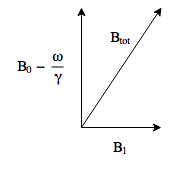
\includegraphics{pythag.png}
 	\caption{In the rotating reference frame the effective field is a vector sum.}
  	\label{fig:boat1}
	\end{figure} 
	
	% Mag Field Trigonometry
	\begin{equation}
	\theta = \arcsin \frac{H_1}{\sqrt{(H_0 - \omega/\gamma)^2 + H_1^2}}
	\end{equation}

	\begin{equation}
	\sin^2(\theta) = \frac{H_1^2}{(H_0 - \omega/\gamma)^2 + H_1^2}
	\end{equation}
	
	\begin{equation}
	\cos^2(\theta) = \frac{(H_0 - \omega/\gamma)^2}{(H_0 - \omega/\gamma)^2 + H_1^2}
	\end{equation}
	
	\begin{equation}
	H_{tot} = \sqrt{(H_0 - \omega/\gamma)^2 + H_1^2}
	\end{equation}
	
	
	% Polarization Signal Definition
	
	% Polarization
	\begin{equation}
	S_z = \cos^2(\theta) + \sin^2(\theta) \cos(\gamma H_{tot} t)
	\end{equation}

	
	
	
	
%	Distribution of Fields?
%		.
%		.
%		.

	%
	% Distribution of Fields
	%
	
	% . 
	
	% .
	 
	% . 
	
	% Histograms
	\begin{equation}
	p(x) = \frac{1}{ { \sigma \sqrt { 2 \pi } } }
	e^{{{ - \left( {x -  \overline{H}_0  } \right)^2 } \mathord{\left/ {\vphantom {{ - \left( {x -  \overline{H}_0 } \right)^2 } {2\sigma ^2 }}} 	\right. 	\kern-\nulldelimiterspace} {2\sigma ^2 }}}
	\end{equation}

\section{\label{sec:level1}Simulation}

%Simulation
%	How does the script calculate the RF Magnetic Field. 
%		.
%		.
%		.
%	How does the script calculate the Polarization signal.
%		.
%		.
%		.
%	How does the script account for distributions in the fields?
%		.
%		.
%		.

	% Introduction to the package
	Simulation of the magnetic field produced by an RF coil was conducted with the python programming language. The simulation was written with adaptability in mind and adheres to well known computational physics practices. Along with vanilla python, the Scipy stack was included. Scipy is a python language enhancement library including functionality for working with data, array based numerical computation and graphical capabilities. The specific libraries included in the simulation were matplotlib (graphics), numpy (numerical computing) and Scipy (scientific functionality). 
	
	% Explanantion of the various components and functionality
	A set of five scripts was produced to simulate the coil. The scripts follow a logical data flow hierarchy and are arranged by functionality. The first script, physics.py, is responsible for defining all equations necessary for calculation as numerical constants utilized throughout the programs life cycle. Among these constants are the physical constants defined for each equation, time and frequency values used for plotting and geometrical considerations of the coil. Two scripts distribution.py and histogram.py are responsible for both calculation the magnetic field distributions and creating histograms of each magnetic field respectively. The fourth script main.py calculates the polarization signal and the fifth script plot.py plots quantities of interest. The inner working of each of these scripts is explained at depth in the appendix of this article. 
	
	\begin{figure}[H]
 	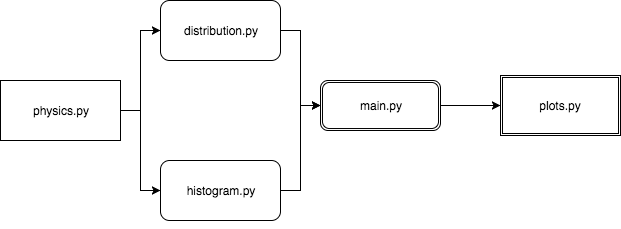
\includegraphics[width=\linewidth]{programOutline.png}
 	\caption{Description of the coil geometry.}
  	\label{fig:boat1}
	\end{figure}
	
	It is assumed that the coil to be simulated follows a rectangular geometry. Such a geometry is defined by it vertical and horizontal stacks of wires. An mxn geometry defines the coil computationally where m is the number of vertical coils and n the number of horizontal coils. It is further assumed that wire of a diameter of 1mm is used and material properties of each turn of wire are equivalent. 
	
	\begin{figure}[H]
 	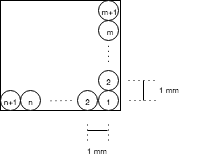
\includegraphics[width=\linewidth]{coil2.png}
 	\caption{Description of the coil geometry.}
  	\label{fig:boat1}
	\end{figure}
	
	%% In depth explanation of algorithm for distribution and histogram provided in appendix. 
	% Explanation of the modular nature of the program
	
	% How to calculate the signal
	\begin{equation}
	\overline{S_z}(H_0) = \frac{1}{\sum p(H_0)p)(H_1)}\sum S_z p(H_0) p(H_1)
	\end{equation}
	
	
	Two coil sets A and B contain n x m windings each. They are each positioned at a distance $z\pm\frac{h}{2}$ from the origin. The radius $R$ is the distance between the individual winding of the coil.

	
	
The model assumes a separation of $1mm$ between the centres of each coil as shown in figure 2. The initial winding for each coil has a radius of $25mm$ and a separation of $25mm$ exists between the two initial windings of coil A and B.

	
	
This model is implemented using the python programming language. 
	
\section{\label{sec:level1}Results}

	\subsection{\label{sec:level2} Derivatives}
	
	A comparison of the derivatives were plotted using the numpy and matplotlib packages from python. Figure 3 shows that the maximum field along the axis of the solenoid for two 5x5 coils is roughly 12 Gauss.
        
        \begin{figure}
            \centering
            \begin{subfigure}[b]{0.3\textwidth}
                \centering
                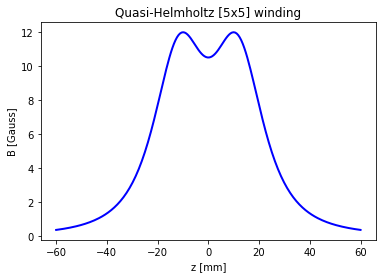
\includegraphics[width=\textwidth]{mag0.png}
                \caption{The Field Distribution (the zeroth derivative.)}
                \label{fig:y equals x}
            \end{subfigure}
            \hfill
            \begin{subfigure}[b]{0.3\textwidth}
                \centering
                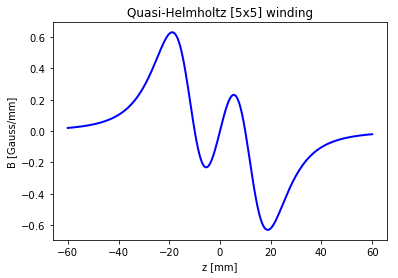
\includegraphics[width=\textwidth]{mag1.png}
                \caption{First derivative of the field distribution}
                \label{fig:three sin x}
            \end{subfigure}
            \hfill
            \begin{subfigure}[b]{0.3\textwidth}
                \centering
                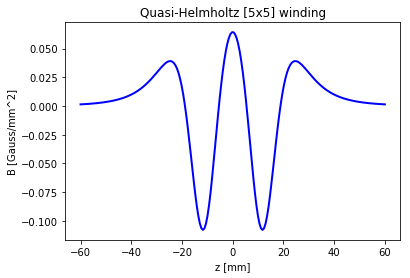
\includegraphics[width=\textwidth]{mag2.png}
                \caption{Second derivative of the field distribution.}
                \label{fig:five over x}
            \end{subfigure}
            \caption{Comparison of the derivatives for the Biot-Savart Law.}
            \label{fig:three graphs}
        \end{figure}
	\subsection{\label{sec:level2} Radial Distribution}
	
	When assessing a radial distribution of the field a sample volume of dimensions $r=2.5mm$ and $thickness=0.5mm$ was considered. The radial distribution is considered at 3 significant points within this sample volume: the left edge, the right edge and the centre.

As was expected, the maximum magnitude of the magnetic field at the center of the sample volume is lower than at the edges (as they are closer to the center of the coils.) However, it was confirmed that in either case the field magnitude decreased radially outwards from the center of the sample.

   \begin{figure}
            \centering
            \begin{subfigure}[b]{0.3\textwidth}
                \centering
                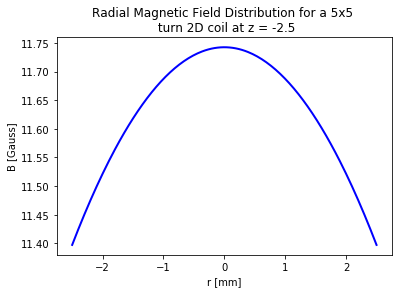
\includegraphics[width=\textwidth]{radneg25.png}
                \caption{Radial distribution at the left sample edge.}
                \label{fig:y equals x}
            \end{subfigure}
            \hfill
            \begin{subfigure}[b]{0.3\textwidth}
                \centering
                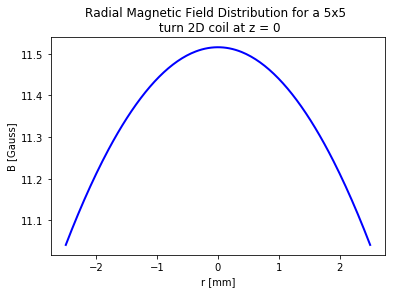
\includegraphics[width=\textwidth]{rad0.png}
                \caption{Radial distribution in the centre of the sample}
                \label{fig:three sin x}
            \end{subfigure}
            \hfill
            \begin{subfigure}[b]{0.3\textwidth}
                \centering
                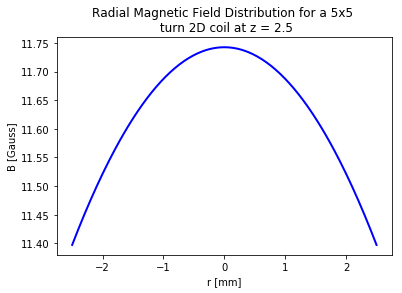
\includegraphics[width=\textwidth]{rad25.png}
                \caption{Radial distribution at the right sample edge.}
                \label{fig:five over x}
            \end{subfigure}
            \caption{Radial distribution at several points in the sample volume.}
            \label{fig:three graphs}
        \end{figure}

	Equations:
		% Diagrams Here

	\begin{figure}

   		\centering
    		\begin{subfigure}[h]{0.4\textwidth}
        			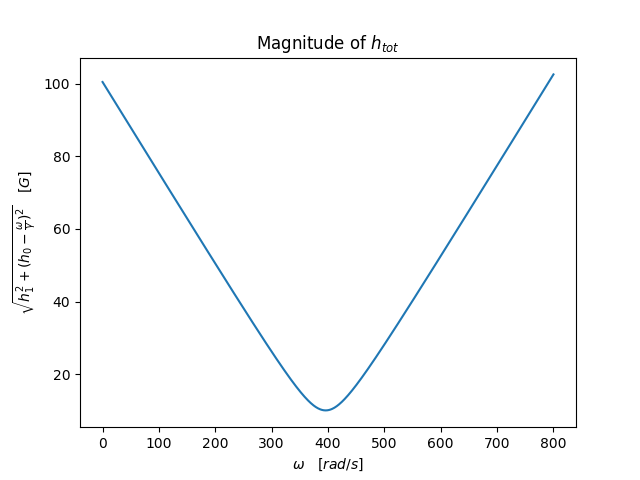
\includegraphics[width=\textwidth]{magnitude-h_tot.png}
        			\caption{Figure 1: Magnitude of the total magnetic field at a distribution of frequencies.}
        			\label{fig:gull}
   		 \end{subfigure}

   	  %add desired spacing between images, e. g. ~, \quad, \qquad, \hfill etc. 
    		  %(or a blank line to force the subfigure onto a new line)

    		\begin{subfigure}[h]{0.4\textwidth}
      	 		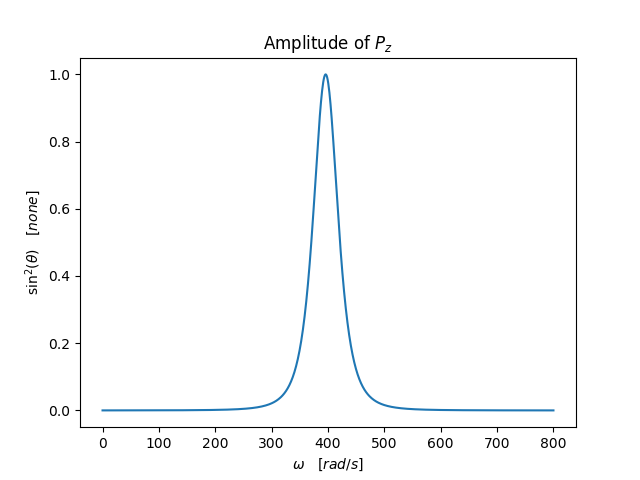
\includegraphics[width=\textwidth]{amplitude-p_z.png}
       	 		\caption{Figure 2: Magnitude of the amplitude for the polarization signal at a distribution of 								frequencies.}
       	 		\label{fig:tiger}
		\end{subfigure}	

	\end{figure}

	\begin{figure}

		\centering
		\begin{subfigure}[h]{0.4\textwidth}
			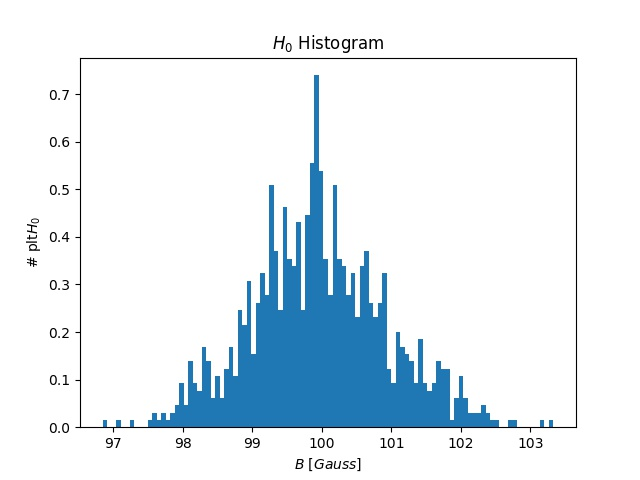
\includegraphics[width=3.5in]{hist_h_0.jpg}
			\caption[Gaussian of $H_0$ on resonance]
			{Probability distribution of magnetic field $H_0$ for $\omega$ = $\gamma H_0$.}
		\end{subfigure}

		\begin{subfigure}[h]{0.4\textwidth}
			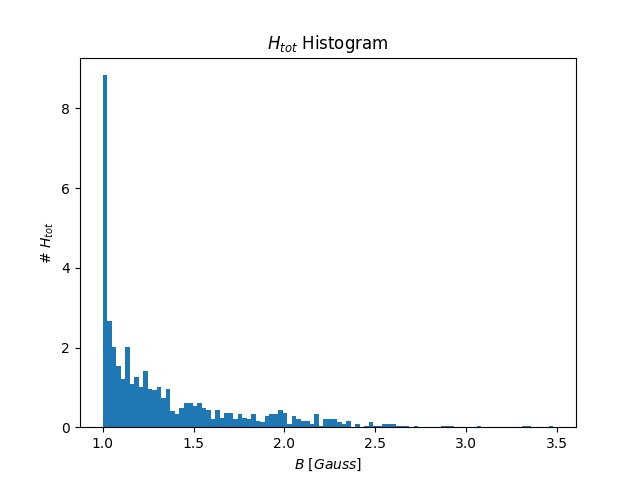
\includegraphics[width=3.5in]{hist_h_tot.jpg}
			\caption[Gaussian of $H_0$ on resonance]
			{Probability distribution of magnetic field $H_{tot}$ for $\omega$ = $\gamma H_0$.}
		\end{subfigure}

	\end{figure}

	\begin{figure}

   		\centering
    		\begin{subfigure}[h]{0.4\textwidth}
      	 		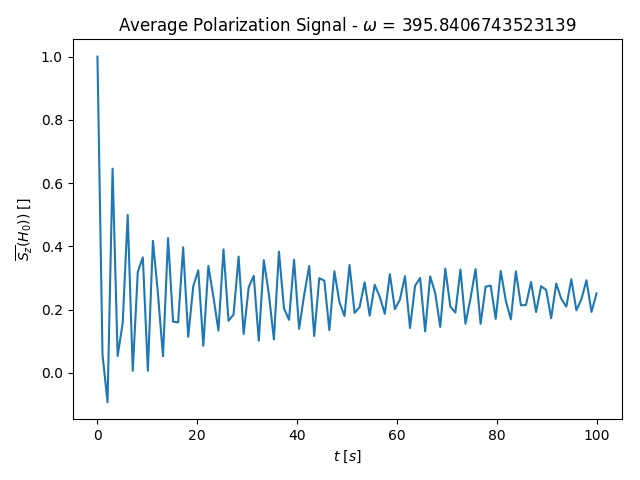
\includegraphics[width=\textwidth]{average_signal.jpg}
       	 		\caption{Figure 4: Average polarization signal for $\omega$ = $\gamma H_0$.}
       	 		\label{fig:tiger}
		\end{subfigure}

	\end{figure}
	
		Parameters:

	\begin{align} 
	H_1 &= 10 \\
	\overline{H}_0 &= 100 \\
	\omega &= h_0 \gamma  \\
	\sigma &= 1 \\
	\end{align}

	
	
\section{\label{sec:level1}Appendix}
	
	The following examines the how the magnetic field due to an individual coil is calculated. 
	
	\begin{equation}
	B(z) = \frac{\mu_0I}{2}\frac{(R+\epsilon)^2} {((R+\epsilon)^2+(z+\tau + offset)^2)^{(3/2)}}
	\end{equation}
	


\end{document}
%
% ****** End of file apssamp.tex ******
